\documentclass[b5paper,12pt]{book}
\usepackage[T1]{fontenc}
\usepackage[utf8]{inputenc}
\usepackage{graphicx}
\usepackage[cc]{titlepic} %MYND Á TITILSÍÐU
\usepackage{xcolor}
\usepackage[icelandic]{babel}
\selectlanguage{icelandic}
%\usepackage{tgtermes}
\usepackage{lmodern}
\renewcommand*\familydefault{\sfdefault} %% Only if the base font of the document is to be sans serif
\usepackage[T1]{fontenc}
\usepackage[export]{adjustbox}
\usepackage{forest}
\usepackage{amsmath,amssymb,amsthm,textcomp,gensymb}
\usepackage[shortlabels]{enumitem} % Gerir mögulegt að nota begin{itemize}[label=$\square$] og [(a)] í enumerate
\usepackage{multicol}
\usepackage{pgf,tikz}
\usetikzlibrary{graphs, graphs.standard, arrows, shapes, trees, snakes}
\usetikzlibrary{automata,positioning,calc}
\usepackage{wrapfig}
\usepackage{hyperref}
\hypersetup{
    colorlinks=true,
    linkcolor=blue,
    filecolor=magenta,      
    urlcolor=red,
}
\usepackage{wasysym} % Einhver tákn, ekki viss hvort bæti við gensymb
\usepackage{geometry}
\geometry{total={210mm,297mm},
left=25mm,right=25mm,%
bindingoffset=0mm, top=20mm,bottom=20mm}
\usepackage{caption}
\usepackage{subcaption}
\usepackage[export]{adjustbox} % Veit ekki hvað þetta gerir
\usepackage{mathrsfs} % Ekki heldur, eitthvað með fonta á stærðfræði
%\usepackage[misc]{ifsym} %Teningatákn, ekki viss hvort bæti við gensymb

\usepackage{multiaudience} % Til að gera kennaraútgáfu og nemendaútgáfu
% Define the possible audiences
\SetNewAudience{kennari}
%Notkun:
%\begin{shownto}{kennari}
%Texti fyrir kennara
%\end{shownto}



\linespread{1.2}

\newcommand{\linia}{\rule{\linewidth}{0.5pt}}

% my own titles
%\makeatletter
%\renewcommand{\maketitle}{
%\begin{center}
%\vspace{2ex}
%{\huge \textsc{\@title}}
%\vspace{1ex}
%\\
%\linia\\
%\end{center}
%}
%\makeatother
\renewcommand*\thesection{\arabic{section}}
\pagestyle{empty}



%Félagsleg tengslanetagreining er notuð á ýmsum fræðasviðum og er í dag lykiltækni í nútíma félagsfræði. (Litlir heimar: Áhrif erlendrar reynslu stjórnenda á viðhorf til notkunar tengslaneta Erla Hjördís Gunnarsdóttir og Magnús Þór Torfason)
%
%Allir kaflar eru verkefni, en þá er hægt að hafa suma kafla sem "lestrarverkefni", texti, skýringar, en alltaf spurning/spurningar.
%
%Byggt upp þannig að hápunktur sé sönnun á friendship paradox.
%
%TO-DO:
% Skrifa um muninn á stærðfræðilegum verkefnum og "hagnýtu". T.d. að sanna að Euler formúlu (stæ) og svo um eiginleika sósíal neta (hagn).
%


\title{\Huge Netafræði: verkefnahefti}
\author{Ingólfur Gíslason}
\date{Útgáfa 0.95 (\the\year)}
\titlepic{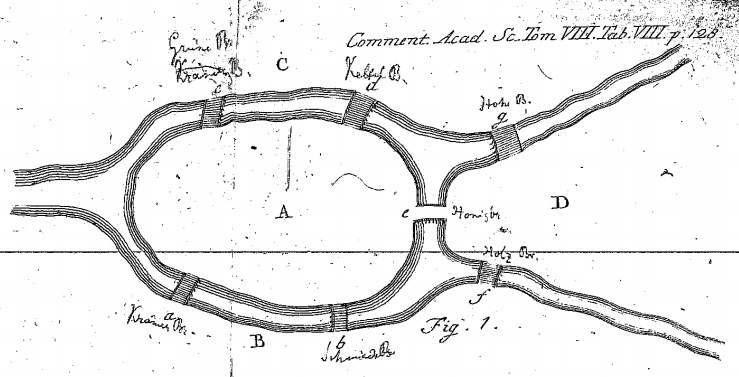
\includegraphics[width=0.7\textwidth]{konigsb_euler.png}}

\begin{document}
\maketitle

\vspace*{\fill}
\begin{minipage}[b]{0.9\textwidth}
\footnotesize\raggedright
\setlength{\parskip}{0.5\baselineskip}
\copyright \the\year\ Ingólfur Gíslason. Hefti þetta má hver sem er nota og deila en ekki eigna sér, breyta eða taka gjald fyrir.   
\end{minipage}

\frontmatter
\pagestyle{plain}
\chapter{Um þetta hefti} 
Þetta hefti er hugsað fyrir byrjendur í framhaldsskólum, á félags- og hugvísindabrautum. Ef nemendur glíma einnig við verkefni merkt „áskorun“ gæti það líka hentað náttúruvísindabrautum. Gert er ráð fyrir því að nemendur vinni saman og með kennara sem hefur góða þekkingu á efninu. Hins vegar er ekki er ætlast til að kennari segi nemendum fyrirfram hvernig eigi að leysa verkefnin. Ekki er gert ráð fyrir neinni sérstakri fyrirfram stærðfræðiþekkingu af hálfu nemenda. Verkefnin eru samt sem áður ekki auðveld og það á ekki að leysa þau hratt og örugglega heldur eiga þau að gefa nemendum færi á því að búa til stærðfræði í samvinnu sín á milli og með kennara. Mikilvægt er að gefa sér góðan tíma og líta ekki á verkefnin eins og venjuleg reiknisdæmi til að klára heldur eitthvað til að dvelja við, tala um, pæla í, læra af, og njóta.\\

\noindent
Þeir nemendur sem leggja sig vel fram um að skilja verkefnin til fullnustu eiga eftir það að hafa öðlast þekkingu og skilning á frumhugtökum netafræðinnar og nokkrum reglum úr talningarfræði auk þess sem þeir eiga að hafa öðlast reynslu og þekkingu á vinnubrögðum stærðfræðinnar, sér í lagi: 
\begin{itemize}
    \item að draga út eiginleika (e. to abstract)
    \item að setja fram og meta tilgátur
    \item að lesa skilgreiningar og setja fram skilgreiningar
    \item að setja fram aðstæður með stærðfræðilíkani 
    \item að lesa og setja fram eigin röksemdarfærslur (sannanir)
\end{itemize}

\noindent
Ekki er gert ráð fyrir að nemendur þurfi meiri texta en þann sem er í heftinu til að fást við verkefnin og læra af þeim, en það getur verið mikilvægt að hafa í huga „góðar vinnuvenjur“ í stærðfræði. Til að leysa verkefnin getur til dæmis verið gagnlegt að 
\begin{itemize}
    \item finna leiðir til að skrásetja eða setja fram á gagnlegan hátt,
    \item skilgreina gagnleg hugtök,
    \item setja fram tilgátur, 
    \item ræða, rökstyðja eða gagnrýna og endurskoða tilgáturnar,
    \item útskýra og sanna niðurstöður eins vel og hægt er,
    \item alhæfa og útvíkka: finna eins almennar reglur og hægt er, tengja við eldri dæmi og fyrri þekkingu,
    \item spyrja nýrra og flóknari spurninga.
\end{itemize}

\noindent
Í fyrsta hluta bókarinnar eru verkefni, en í seinni hlutanum eru athugasemdir og vísbendingar um nokkur dæmanna. Í kennarabók (ekki til eins og er) verða svo meiri upplýsingar um lausnir dæmanna. 

\mainmatter
\pagestyle{plain}
\setcounter{page}{1}
\pagenumbering{arabic}
%\addtocounter{chapter}{1}
\chapter*{Verkefni í netafræði} 
\section{Tengslanet}
\label{sec:fyrstanet}
Anna er vinur Bjarna, Dóru og Einars. Bjarni er vinur Clöru. Clara er vinur Dóru og Finns. Finnur er vinur Einars. Dóra er vinur Einars og Finns.
\begin{enumerate}[(a)]
    \item Hver á flesta vini?
    \item Hve mörg vináttutengsl eru í þessu tengslaneti? Önnur leið til að orða spurninguna væri: hvað eru mörg vinapör?
    \item Hvað eiga stelpurnar marga strákavini að meðaltali, og hvað eiga strákarnir marga stelpuvini að meðaltali?
    \item Ein forsenda dæmisins var hugsuð þannig: ef $A$ er vinur $B$ þá er $B$ sjálfkrafa vinur $A$. Það er líka hægt að gera ráð fyrir að svo sé ekki, en þá er dæmið bara öðruvísi. Eru fleiri óorðaðar forsendur í dæminu?
    \item Flettið upp á lausnarleiðum í kaflanum \nameref{chap:frodleikur}.
\end{enumerate}

\section{Möguleg og ómöguleg tengslanet}
Teiknið dæmi um tengslanet ef það er hægt, annars ekki:
\begin{enumerate}[(a)]
    \item Það eru fjórir einstaklingar og allir eru vinir allra. 
    \item Það eru fimm einstaklingar og allir eiga nákvæmlega tvo vini.
    \item Það eru fimm einstaklingar og einn þeirra á fjóra vini en hinir eiga allir bara einn vin.
    \item Nákvæmlega þrír einstaklingar eiga nákvæmlega þrjá vini.
\end{enumerate}

\section{Net, hnútar og leggir}
Teiknað hefur verið tengslanet þar sem bókstafir í hringjum tákna einstaklinga og þeir tengjast ef þeir eru vinir. Í netafræði er hefð fyrir því að tala um hringina (stundum táknað með punktum) sem \textbf{hnúta} (e. vertex eða node) og strikin sem \textbf{leggi} (e. edge eða link). Saman mynda hnútarnir og leggirnir \textbf{net} (e. graph eða network). 
\begin{figure}[h]
    \centering
\begin{tikzpicture}
    \graph[nodes={draw, circle}, n=5, clockwise,radius=1.5cm]{subgraph C_n [V={A,B,C,D,E}];};
    \node[shape=circle,draw=black] (F) at (0,0) {F};
    \path [-](F) edge node {} (A);
    \path [-](F) edge node {} (B);
    \path [-](F) edge node {} (C);
    \path [-](F) edge node {} (D);
    \path [-](F) edge node {} (E);
\end{tikzpicture}
\caption*{Netið fyrir verkefni \thesection{}.}
\end{figure}

\begin{enumerate}[(a)]
    \item Hve margir hnútar eru í netinu?
    \item Hve margir leggir eru í netinu?
    \item Einhver utanaðkomandi vill koma skilaboðum til allra í netinu, og ætlar að fá einhvern til að pósta á samfélagsmiðil. Hvern ætti hann að velja? 
    \item Ef einhver hópur þekkist innbyrðis, allir þekkja alla hina, er það nefnt \textbf{klíka}. Til að auka nákvæmnina er líka talað um \textbf{3-klíkur}, ef þrír eru í klíkunni, \textbf{4-klíkur} ef fjórir eru í klíkunni og svo framvegis. Hve margar ólíkar 3-klíkur eru í netinu og hve margar 4-klíkur eru í netinu?
\end{enumerate}

\section{Að draga út eiginleika}
Stærðfræði er notuð þannig að raunverulegum (eða ímynduðum) aðstæðum er breytt í stærðfræði. Svo er unnið með stærðfræðina, og að lokum er stærðfræðilausnin túlkuð yfir í aðstæðurnar. Fyrsta skrefið í þessu ferli er \textbf{að draga út} (e. to abstract) þá eiginleika sem skipta máli fyrir okkur í hvert skipti, en líta framhjá öllu öðru. Þegar tengslanet eru skoðuð, er ein leið að líta framhjá öllu öðru en þessu: hverjir tengjast hverjum? Þá höfum við sleppt því að taka með í reikninginn hvar fólkið er, hverjir eru nálægt öðrum, hvað fólkið er gamalt, hvað það heitir, hvernig það lítur út og svona mætti halda áfram endalaust. Stærðfræðilega framsetningin á þeim eiginleikum sem skipta máli nefnist svo \textbf{stærðfræðilegt líkan}.\\   
Segjum sem svo að öllum innbyrðis vinatengslum í eftirfarandi fjögurra manna hópi af íslenskum unglingum sé rétt lýst með eftirfarandi: Jói er 15 ára og þekkir Söru sem er 16 ára og Sara þekkir Gunnar sem er 17 ára og Gunnar þekkir Hönnu sem er 16 ára og Hanna þekkir Jóa sem talað var um fyrst í þessari upptalningu. 
\begin{enumerate}[(a)]
\item Ef einn vinur byrjar og segir einum vini sínum leyndarmál, og allir sem heyra leyndarmál segja alltaf öllum vinum sínum leyndarmálið daginn eftir að þeir heyra það, hvað tekur langan tíma þangað til allir vinirnir hafa heyrt leyndarmálið? 
\item Hvaða upplýsingar dróstu úr lýsingunni og notaðir til að búa til stærðfræðilegt líkan í lið a? Hvaða upplýsingar notaðir þú ekki?
\item Hver er elstur og hver er yngstur af þessum unglingum? 
\item Hvaða upplýsingar dróstu úr lýsingunni og notaðir til að búa til stærðfræðilegt líkan í lið c? Hvaða upplýsingar notaðir þú ekki?
\end{enumerate}

\section{Kynlíf}
\label{sec:gagnkyn}
Í rannsóknum á (gagnkynhneigðri) kynlífshegðun hefur oft komið fram að karlar svara þannig að þeir hafi stundað kynlíf með fleiri konum að meðaltali heldur en konur með körlum. Getur þetta verið rétt? Til að kanna málið er hægt að hugsa sér samfélag með (til dæmis) sex körlum og sex konum, og búa til ólíkar „sviðsmyndir“, það er að segja ólík dæmi um hugsanleg (gagnkynhneigð) kynlífstengsl innan þessa hóps. 

\section{Eins net}
Þegar net eru teiknuð skiptir ekki máli hvernig netið snýr eða nákvæmlega hvar hnútarnir eru, heldur aðeins hvaða hnútar eru tengdir saman með leggjum. Þess vegna geta mismunandi teikningar táknað sama netið. Hvaða teikningar tákna sama netið?
\begin{figure}[h]
  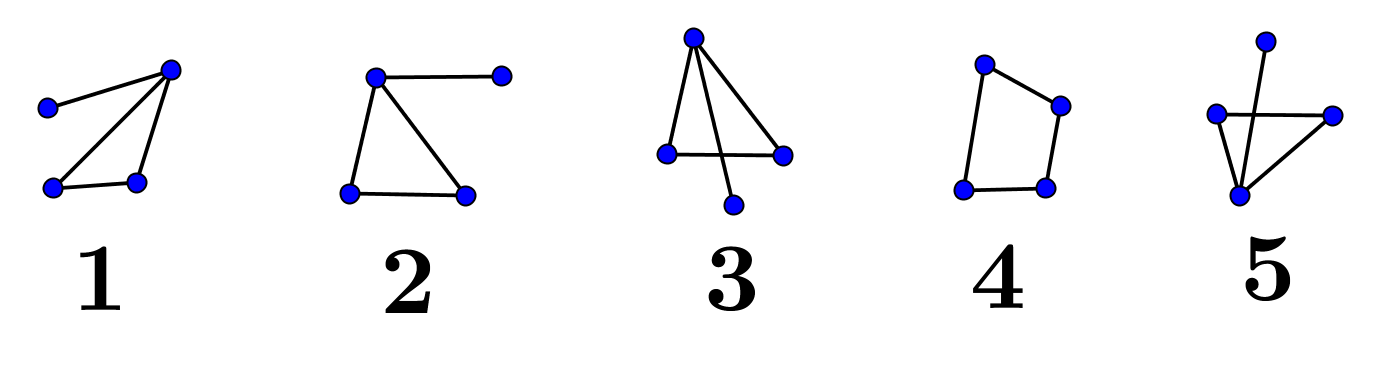
\includegraphics[width=0.75\textwidth, center]{einsnet.png}
  \caption*{Hvaða net eru eins í verkefni \thesection{}?}
\end{figure}

\section{Leikur: búum til tengslanet}
Hér þarf að vera einhver hópur af nemendum. Notið leikinn „steinn, pappír eða skæri“. Sérhverjir tveir nemendur spila einu sinni. Ef útkoman er jafntefli þá tengjast þeir ekki, annars tengjast þeir. Það má líka nota aðra leiki, til dæmis að kasta upp peningi, eða teningum og vissar summur þýða tengingu en aðrar ekki. Teiknið upp svona tengslanet.  
\begin{enumerate}[(a)]
    \item Er netið samhangandi eða myndast „eyjur“? (\textbf{Samhangandi} þýðir að sama hvaða tveir hnútar eru valdir, það er einhver „leið“ (listi af leggjum) sem tengir þá.)  
    \item Hverjir eru „mikilvægastir“ fyrir útbreiðslu upplýsinga? Af hverju?
    \item Eru einhverjir í netinu þannig að ef þeir væru teknir burt þá myndi netið slitna?
    \item Hve margar 3-klíkur eru í netinu og hve margar 4-klíkur eru í netinu?
\end{enumerate}

\section{Vinaþversögnin}
\label{sec:vina}
Markmiðið í þessu dæmi er að skoða fullyrðinguna \textbf{„að meðaltali eiga vinir manns fleiri vini en maður sjálfur“}. Fyrst skoðum við lítið ímyndað dæmi um vinatengsl sem netið á myndinni lýsir (hnútar tákna fólk, leggur á milli táknar að manneskjurnar eru vinir). 
\begin{figure}[h!]
\centering
\begin{tikzpicture}
   \node[shape=circle,draw=black] (A) at (0,0) {A};
    \node[shape=circle,draw=black] (B) at (0,3) {B};
    \node[shape=circle,draw=black] (C) at (2.5,4) {C};
    \node[shape=circle,draw=black] (D) at (2,2) {D};
    \node[shape=circle,draw=black] (E) at (2.5,-1) {E};
    \node[shape=circle,draw=black] (F) at (5,3) {F} ;
    %\path [->](A) (B); 
    \path [-](A) edge node {} (B);
    \path [-](B) edge node {} (C);
    \path [-](A) edge node {} (D);
    \path [-](D) edge node {} (C);
    \path [-](A) edge node {} (E);
    \path [-](D) edge node {} (E);
    \path [-](D) edge node {} (F);
    \path [-](C) edge node {} (F);
    \path [-](E) edge node {} (F); 
\end{tikzpicture}
\caption*{Net fyrir verkefni \thesection{}.}
\end{figure}
\begin{enumerate}[(a)]
    \item Finnið hvað hver manneskja á marga vini.
    \item Reiknið meðalfjölda vina í þessu tengslaneti. (Hvað á hver manneskja marga vini að meðaltali?)
    \item Reiknið út hvað vinir B eiga marga vini að meðaltali. 
    \item Reiknið út hvað vinir F eiga marga vini að meðaltali. 
    \item Haldið áfram og kannið hvort þessi fullyrðing er sönn: „Að meðaltali eiga vinir manns fleiri vini en maður sjálfur“.
    \item \textbf{Áskorun:} Sýnið fram á að niðurstaða ykkar í síðasta lið á við um öll tengslanet [þetta er \underline{mjög} krefjandi verkefni]. 
\end{enumerate}
Það gæti verið áhugavert að búa til fleiri dæmi og/eða reyna að rannsaka þetta mál nánar. Fullyrðingin er vel þekkt og hægt er að finna efni um hana á netinu með því að gúgla
\href {http://www.google.com/search?q="friendship paradox"}{„friendship paradox“}.

\section{Einn sameiginlegur vinur}
\begin{enumerate}[(a)]
\item Hvaða pör af einstaklingum eiga nákvæmlega einn sameiginlegan vin í hópnum, samkvæmt tengslanetinu sem teiknað er?

\begin{figure}[h]
    \centering
\begin{tikzpicture}
    \graph[nodes={draw, circle}, n=8, clockwise,radius=1.5cm]{A, B, C, D, E, F, G, H};
    \node[shape=circle,draw=black] (I) at (0,0) {I};
    \path [-](I) edge node {} (A);
    \path [-](I) edge node {} (B);
    \path [-](I) edge node {} (C);
    \path [-](I) edge node {} (D);
    \path [-](I) edge node {} (E);
    \path [-](I) edge node {} (F);
    \path [-](I) edge node {} (G);
    \path [-](I) edge node {} (H);
    \path [-](A) edge node {} (B);
    \path [-](C) edge node {} (D);
    \path [-](E) edge node {} (F);
    \path [-](G) edge node {} (H);
\end{tikzpicture}
\caption*{Netið fyrir verkefni \thesection{}.}
\end{figure}
\item Teiknið tengslanet 7 einstaklinga með þennan eiginleika: sérhverjir tveir einstaklingar í netinu eiga nákvæmlega einn sameiginlegan vin.
\end{enumerate}

\section{Karateklúbburinn}
Í mannfræðirannsókn (Zachary, 1977: \textit{An Information Flow Model for Conflict and Fission in Small Groups}) var búið til líkan af því hvernig upplýsingar og skilaboð streymdu þegar ágreiningur varð og hópar sundruðust innan karateklúbbs í Bandaríkjunum. Í klúbbnum voru 34 einstaklingar og í fræðilegu greininni sem rituð var um rannsóknina birtist net sem sýndi tengslin milli þeirra. Einstaklingar töldust hafa tengsl ef þeir höfðu regluleg samskipti utan klúbbsins.  

\begin{figure}[h]
  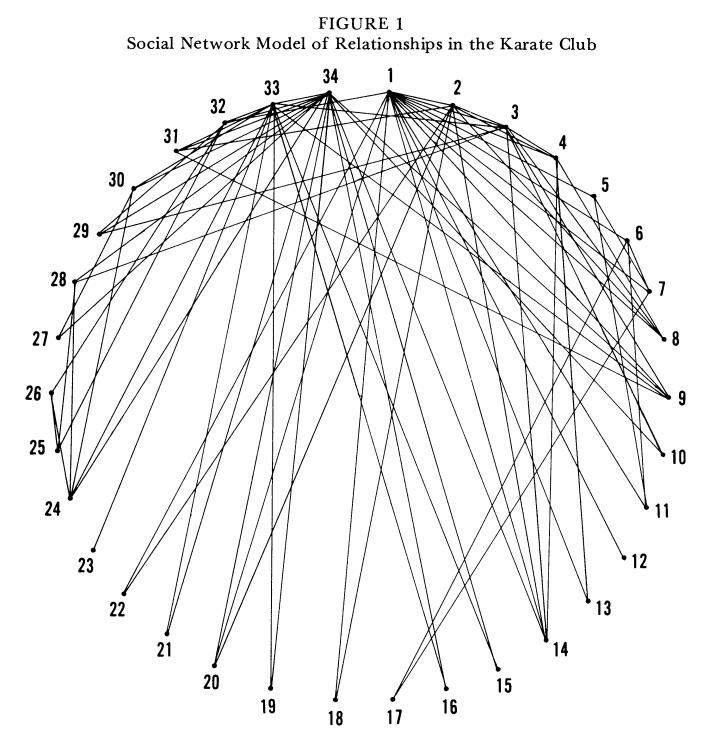
\includegraphics[width=0.75\textwidth, center]{Karateclub.png}
  \caption*{Tengslanet í karateklúbbnum.}
\end{figure}

\begin{enumerate}[(a)]
    \item Er hægt að segja eitthvað út frá myndinni um það hverjir eru „mikilvægustu“ einstaklingarnir, út frá félagslegu sjónarmiði? 
    \item Rifjum upp að fjöldi leggja sem tengjast hnúti nefnist \textbf{gráða} hnútarins. Hverjar eru gráður hnúta númer 19, 20, 21, 22, og 23?
    \item Hvaða hnútar virðast hafa hæstu gráðurnar?
\end{enumerate}

\section{Tafla (eða fylki)}
Í síðasta verkefni var mynd af neti sem erfitt er að lesa af þar sem það er þéttast. Ein hefðbundin leið til þess að setja fram net (og til að „geyma“ upplýsingar um net, til dæmis í tölvum) er að búa til töflu. Taflan telur alla hnúta fylkisins í einum dálki og líka í röð. Ef hnútur númer $n$ tengist hnúti númer $m$ er talan 1 sett í hólfið í dálki $n$ og röð $m$ (og líka í dálki $m$ og röð $n$), en annars er sett 0. 

\begin{figure}[h]
  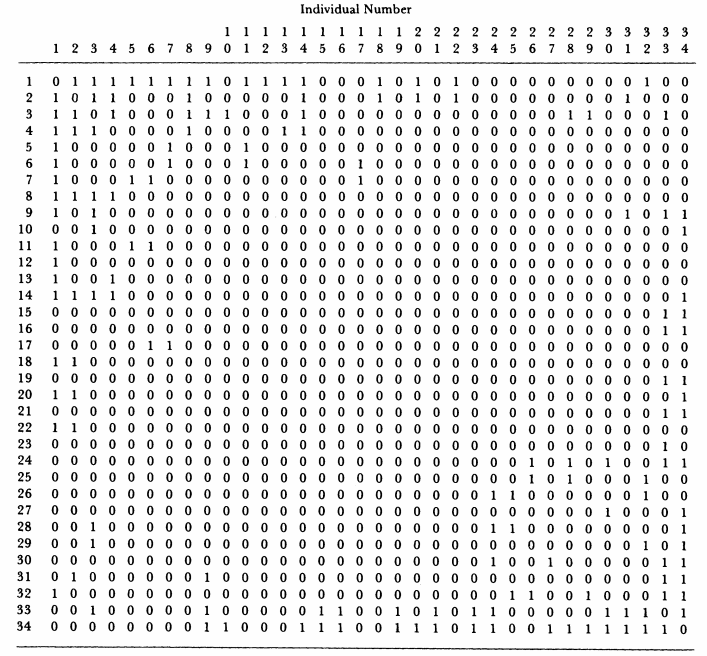
\includegraphics[width=0.75\textwidth, center]{Karatetafla.png}
  \caption*{Fylkið fyrir tengslanet í karateklúbbnum.}
\end{figure}

Töflur eins og þessar nefnast \textbf{fylki} í stærðfræði, í netafræði heitir svona tafla \textbf{hnútafylki} netsins. Sýnum fylki fyrir tengslanetið í karateklúbbnum, og notum töfluna til að svara spurningunum:
\begin{enumerate}[(a)]
    \item Finnið gráður hnúta númer 1, 33 og 34. 
    \item Hvaða tveir hnútar hafa hæstu gráðunar?
    \item Hvað eiga þeir einstaklingar marga sameiginlega vini?
\end{enumerate}

\section{Stutt æfing um hnútafylki}
Það að búa til hnútafylki út frá teikningu af neti (eða öfugt) er dæmi um algengan hlut í stærðfræði: \textbf{að þýða á milli ólíkraframsetninga} (e. representations). Eftirfarandi verkefni eru um það: 
\begin{enumerate}[(a)]
    \item Gerið hnútafylki fyrir netið í verkefninu um vinaþversögnina, verkefni \ref{sec:vina}.
    \item Teiknið netið sem hefur eftirfarandi hnútafylki:

\begin{tabular}{ c | c c c c c } 
      & a & b & c & d & e \\
    \hline
    a & 0 & 1 & 1 & 0 & 0 \\
    b & 1 & 0 & 1 & 1 & 0 \\
    c & 1 & 1 & 0 & 0 & 1 \\
    d & 0 & 1 & 0 & 0 & 0 \\
    e & 0 & 0 & 1 & 0 & 0 
\end{tabular}
\end{enumerate}

%An Information Flow Model for Conflict and Fission in Small Groups

%%%%%%%%%%%%%%%%%%%%%%%%%%%%%%%%%%%%%%%%%%%%%%%%
%%%%%%%%%%%%%%%%%%%%%%%%%%%%%%%%%%%%%%%%%%%%%%%%


\section{Brýrnar í Königsberg}
Hér er mynd af borg. Fljót rennur gegnum borgina og það eru sjö gamlar og fallegar brýr sem tengja borgarhlutana saman. Verkefnið er að hanna gönguferð þannig að farið sé um hverja brú einu sinni og ekki oftar.  

\begin{figure}[h]
  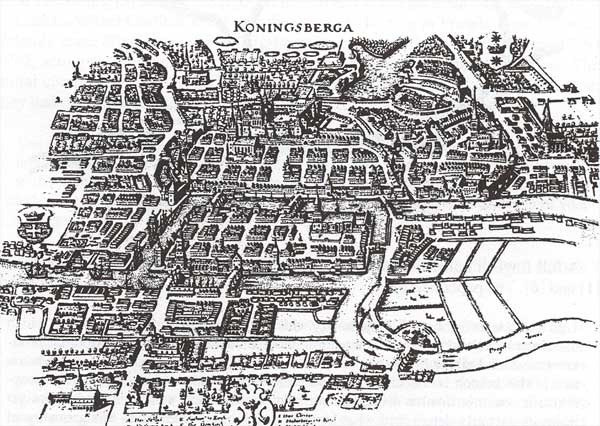
\includegraphics[width=0.75\textwidth, center]{koningbryr.jpg}
  \caption*{Gamalt kort af Königsberg.}
\end{figure}

\noindent
Svissneski stærðfræðingurinn Leonhard Euler (1707–1783) leysti þrautina um brýrnar í Königsberg árið 1735. Greinin sem hann skrifaði um þrautina heitir Solutio Problematis ad Geometriam Situs Pertinentis (Lausn á verkefni um rúmfræði staðsetninga). Euler byrjaði á því sem maður á alltaf að gera, bjó til einfaldaða útgáfu af verkefninu, með því að draga út þá eiginleika sem skipta máli, en sleppa hinum. 

\begin{figure}[h]
  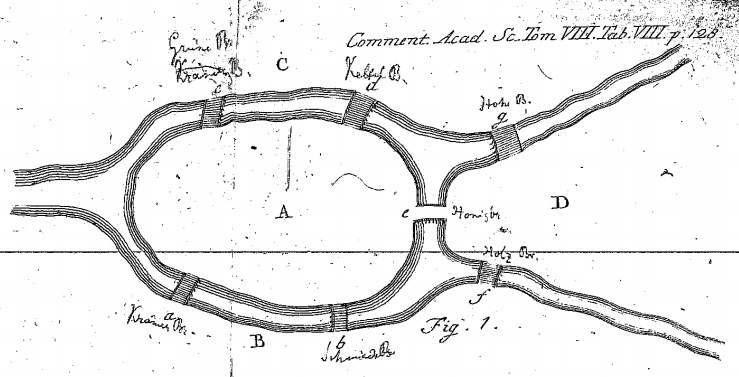
\includegraphics[width=0.75\textwidth, center]{konigsb_euler.png}
   \caption*{Einfölduð teikning Eulers af brúnum í Königsberg.}
\end{figure}

\noindent 
Reynið að finna gönguferð þannig að farið sé yfir hverja brú nákvæmlega einu sinni. Ef það er ekki hægt, reynið að útskýra hvers vegna það er ekki hægt.

\section{Net, hnútar, leggir, rás, tré og gráða hnútar}
Til þess að eiga við verkefni eins og hér á undan (og mörg mörg fleiri) er til stærðfræðikenning sem heitir netafræði (e. graph theory). Frumhugtök kenningarinnar eru net (e. graph), leggur (e. edge) og hnútur (e. vertex). \textbf{Net} er safn af \textbf{hnútum} og \textbf{leggjum} þannig að hver leggur tengist nákvæmlega tveimur hnútum. (Einnig er hægt að hugsa sér legg sem tengist aftur í sama hnút.) Annað heiti sem oft er notað þegar (hluti af) netafræði er hagnýtt í ýmsum greinum er network theory eða network science. Svara á þremur spurningum um þrjú net í þessu verkefni.

\begin{figure}[h]
  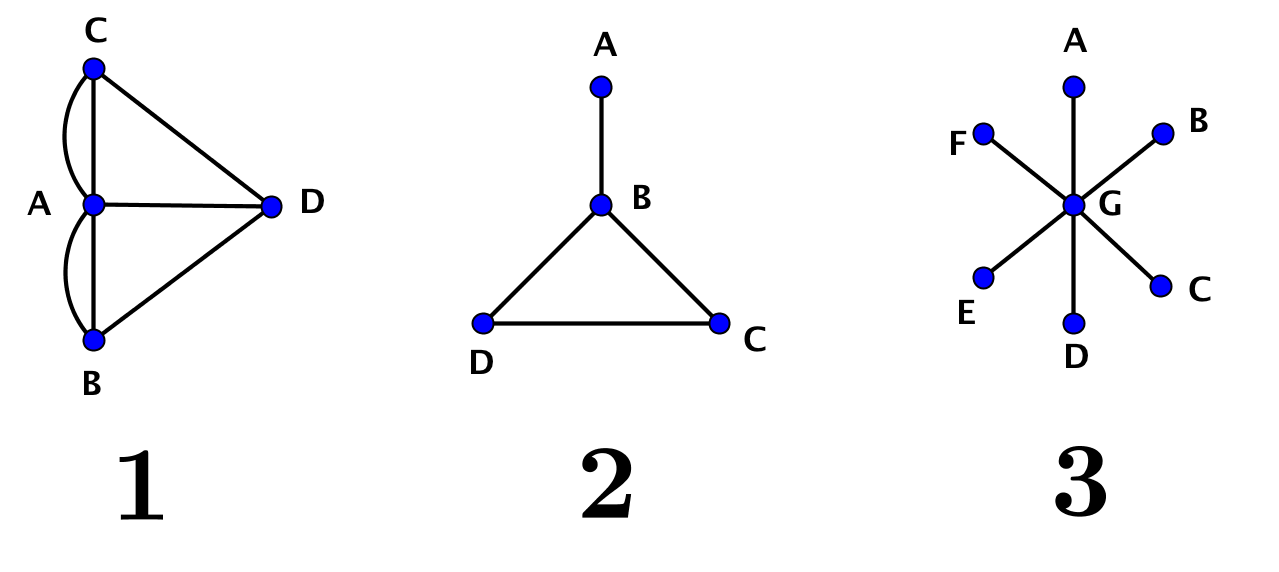
\includegraphics[width=0.7\textwidth, center]{fyrstunet.png}
  \caption*{Netin fyrir verkefni \thesection{}.}
\end{figure}

\begin{enumerate}[(a)]
\item Eitt netið er stærðfræðilegt líkan af brúnum í Köningsberg (sjá að ofan) þar sem hnútur táknar landsvæði en leggur táknar brú. Hvaða net er það?
\item \textbf{Rás} í neti er röð af hnútum og leggjum sem byrja og enda á sama hnúti. Net sem hefur enga rás er kallað \textbf{tré}. Hvaða net hafa rásir og hvaða net er tré?
\item Rifjum upp að \textbf{Gráða hnútar} er fjöldi leggja sem tengjast hnútinum. Í einu netinu hér að ofan er gráða A = 1 og gráða B = 3. Þetta verður líka skrifað með fallarithætti: $g(A)=1$, $g(B)=3$. Hvaða net er þetta?
\item Skráið fjölda leggja í hverju neti. 
\end{enumerate}
 
\section{Heildargráða}
\textbf{Heildargráða nets} er summan af öllum gráðum allra hnúta í netinu.
\begin{enumerate}[(a)]
\item Hverjar eru heildargráður netanna í síðasta verkefni?
\item Hvernig tengist heildargráðan fjölda leggja? (Ef maður telur alla leggina getur maður þá sagt hver heildargráðan er? Ef svo er, hvers vegna?) Þetta er mikilvægt verkefni til að æfa stærðfræðilega röksemdarfærslu.
\end{enumerate}

\section{Sléttir hnútar og oddahnútar}
Ef gráða hnútar er oddatala má kalla þann hnút \textbf{oddahnút} en annars \textbf{sléttan hnút}.
Hvaða hnútar í netum 1, 2 og 3 úr síðustu dæmum hér að ofan eru sléttir hnútar og hverjir eru oddahnútar? 

\section{Möguleg og ómöguleg net}
Teiknið ef hægt er.
\begin{enumerate}[(a)]
\item net sem hefur þrjá slétta hnúta og enga aðra hnúta,
\item net sem hefur þrjá slétta hnúta og einn oddahnút,
\item net sem hefur þrjá slétta hnúta og tvo oddahnúta,
\item net sem hefur þrjá slétta hnúta og þrjá oddahnúta,
\item net sem hefur tvo slétta hnúta og einn oddahnút,
\item net sem hefur tvo slétta hnúta og tvo oddahnút,
\item net sem hefur tvo slétta hnúta og þrjá oddahnúta.
\end{enumerate}

\section{Hvað geta verið margir oddahnútar?}
Skoðið síðasta dæmi, og \textbf{setjið fram tilgátu} um fjölda oddahnúta í hvaða neti sem er.  Getur fjöldi oddahnúta verið hver sem er? Hvaða regla gildir og af hverju? Þetta er mikilvægt verkefni til að æfa stærðfræðilega röksemdarfærslu.

\section{Vegur, Euler-vegur og Euler-rás}
Skoðum aftur eitt af netunum frá því áður:

\begin{figure}[h]
  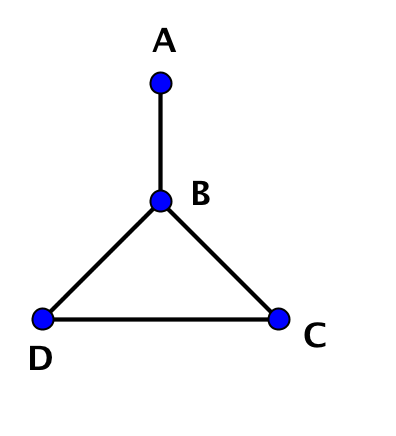
\includegraphics[width=0.2\textwidth, center]{einfaltnet.png}
  \caption*{Netið fyrir verkefni \thesection{}.}
\end{figure}

\begin{enumerate}[(a)]
\item Ef A, B, C, og D tákna staði og leggirnir tákna brýr, er hægt að ferðast þannig að maður fari nákvæmlega einu sinni yfir hverja brú? (Þetta er sama og verkefni Eulers í Königsberg). Hvernig? Finnið alla möguleika.
\item \textbf{Vegur} er listi þar sem skiptast á hnútar og leggir, og hann byrjar og endar á hnútum. Nóg er að gefa upp hnútana. Til dæmis væri ABCBA vegur í netinu hér að ofan (en hann er ekki þannig að maður fari einu sinni um hvern legg!). \textbf{Euler-vegur} er vegur þar sem hver einasti leggur kemur fyrir nákvæmlega einu sinni. Ef Euler-vegur byrjar og endar á sama stað nefnist hann \textbf{Euler-rás}. 
Hefur netið hér að ofan Euler-rás? Hvaða? Finnið þær allar (ef einhverjar eru).
\end{enumerate}

\section{Teikningar án þess að lyfta}
Er hægt að teikna eftirfarandi myndir án þess að lyfta blýantinum eða fara ofan í sama strikið tvisvar? Ef það er hægt: hvernig? Eða með tæknilegu orðalagi: er til Euler-vegur í þessum netum?) Það gæti borgað sig að merkja hnútana með tölum eða bókstöfum, til að hægt sé að skrásetja vegina.

\begin{figure}[h]
  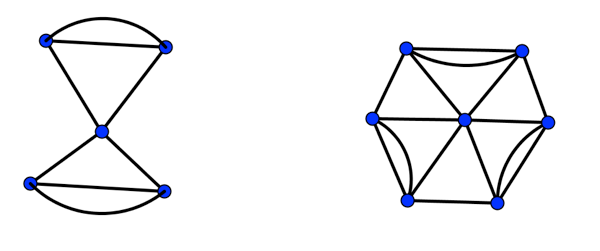
\includegraphics[width=0.5\textwidth, center]{Eulerspurning1.png}
  \caption*{Netin fyrir verkefni \thesection{}.}
\end{figure}

\section{Euler-rásir og Euler-vegir í fjórum netum} Svarið spurningunum um hvert og eitt net.

\begin{figure}[h]
  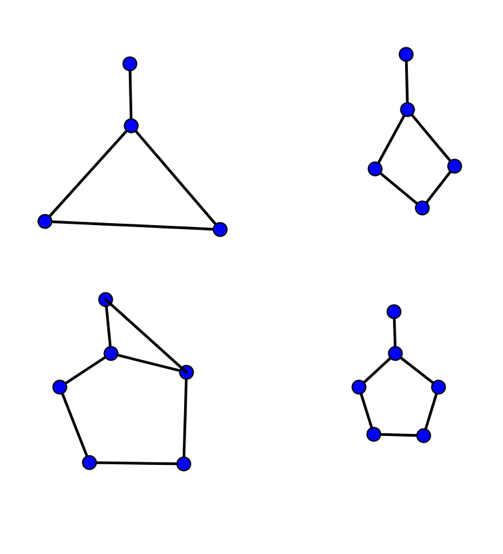
\includegraphics[width=0.4\textwidth, center]{Eulerspurning2.png}
  \caption*{Netin fyrir verkefni \thesection{}.}
\end{figure}

\begin{enumerate}[(a)]
\item Hefur það Euler veg?
\item Hefur það Euler-rás?
\end{enumerate}

\section{Mögulega og ómögulega Euler}
Teiknið ef það er hægt, og segið hvort netin hafa Euler-rás og/eða Euler-veg:
\begin{enumerate}[(a)]
\item net sem hefur þrjá slétta hnúta og enga aðra hnúta,
\item net sem hefur fjóra slétta hnúta og enga aðra,
\item net sem hefur fjóra oddahnúta og enga aðra,
\item net sem hefur tvo oddahnúta og tvo slétta hnúta,
\item net sem hefur tvo oddahnúta og þrjá slétta hnúta.
\end{enumerate}

\section{Regla um Euler--veg}
Finnið reglu sem segir eitthvað um það hvernig net hafa Euler-veg og hvernig net hafa ekki Euler-veg. Rökstyðjið allt sem hægt er. \textbf{Þetta er mikilvægt verkefni!}

\section{Fleiri teikningar}
Er hægt að teikna eftirfarandi myndir án þess að lyfta blýantinum eða fara ofan í sama strikið tvisvar?

\begin{figure}[h]
  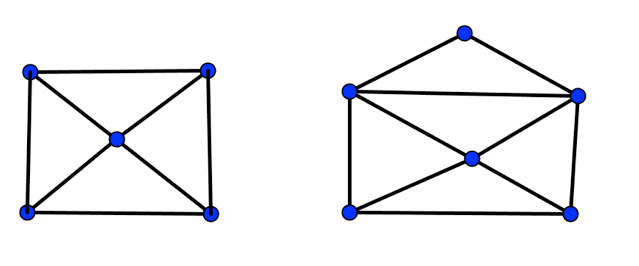
\includegraphics[width=0.5\textwidth, center]{Eulerspurning3.png}
  \caption*{Myndir fyrir verkefni \thesection{}.}
\end{figure}

\section{Um Euler}
Svissneski stærðfræðingurinn Leonhard Euler (1707–1783) leysti þrautina um brýrnar í Königsberg árið 1735. Greinin sem hann skrifaði um þrautina heitir Solutio Problematis ad Geometriam Situs Pertinentis (Lausn á verkefni um rúmfræði staðsetninga). Hann gerði grein fyrir og sannaði fyrstu reglurnar í netafræði, til dæmis um það hvaða net hafa Euler--veg og Euler--rás og þess vegna eru þessi fyrirbæri nefnd eftir honum. Það má segja að hann hafi fundið upp netafræði. Lesið ykkur aðeins til um Leonhard Euler, til dæmis \href {http://www.visindavefur.is/svar.php?id=60127} {umfjöllun Vísindavefsins um Leonhard Euler} og svarið þessum spurningum:
\begin{enumerate}[(a)]
    \item Um það bil hve mörg fræðileg verk gaf Euler út um æfina? 
    \item Hver voru síðustu orð Eulers?
    \item Hve mörg börn eignaðist hann?
\end{enumerate}

\section{Streymi}
\label{sec:streymi}
Á öllum teikningunum hér fyrir neðan táknar B borholu og V táknar vinnslustöð. Leiðslur eru táknaðar með strikum og tölurnar við strikin tákna flutningsgetuna í þúsundum lítra á mínútu. Finna á út hversu mikið af olíu getur (í mesta lagi) streymt frá B til V á mínútu. (Í stað olíu má hugsa sér: hitaveituvatn, gígabæt, eða allt sem getur streymt um einhverskonar farvegi.)
\begin{figure}[h]
  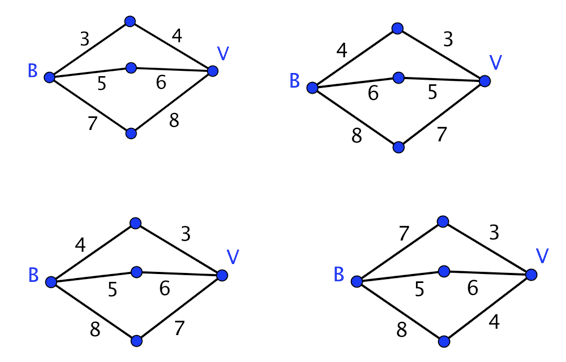
\includegraphics[width=0.6\textwidth, center]{Flaedi1.png}
  \caption*{Netin fyrir verkefni \thesection{}.}
\end{figure}

\section{Sannleikurinn um streymi og þversnið}
Hugtakið \textbf{þversnið} í neti táknar summuna af öllum tölum á leggjunum sem strik sem skiptir netinu í tvennt skarast við. (Þetta er flókin setning sem þarf líklega að lesa aftur.) Á myndinni með þessu verkefni er eitt dæmi um þversnið, sem er jafnt 17. Finnið öll hin þversniðin (allar summurnar). Hvaða þversnið er minnst? 
\begin{figure}[h]
  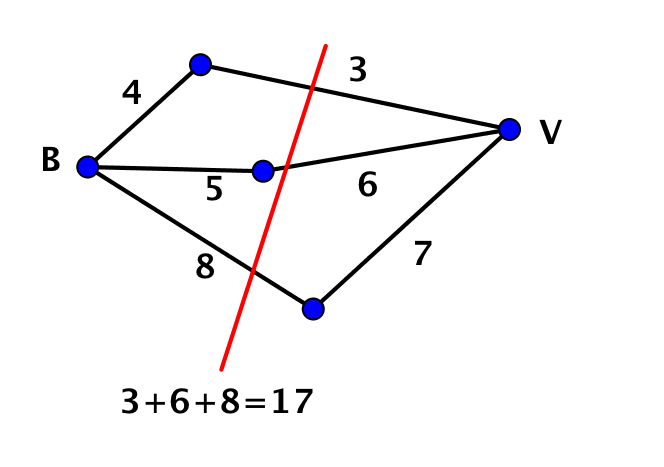
\includegraphics[width=0.4\textwidth, center]{Thversnid.png}
  \caption*{Net fyrir verkefni \thesection{}.}
\end{figure}

Ef þið hafið unnið þetta og síðasta verkefni vel, hafið þið komist að eftirfarandi:\\

\textbf{Mesta streymi í netkerfi er það magn sem flætt getur um minnsta þversniðið.}

\section{Meira streymi}
Bandarísku stærðfræðingarnir Ford og Fulkerson sönnuðu regluna um mesta streymi og minnsta þverskurð (e. max-flow min-cut theorem) árið 1956. (Einnig sönnuðu Elias, Feinstein og Shannon regluna sama ár, óháð Ford og Fulkerson). Aðferð þeirra er notuð í framleiðslugreiningu (e. operations research) og er, fyrir utan reikna stremi af öllum gerðum, meðal annars notuð í verkfræðilegri greiningu á verkefnavali (e. project selection problem) og í tölvusjóntækni (þegar tölvuforrit greina myndir). Spurt er um mesta mögulega streymi í kerfinu sem gefið er.
\begin{figure}[h]
  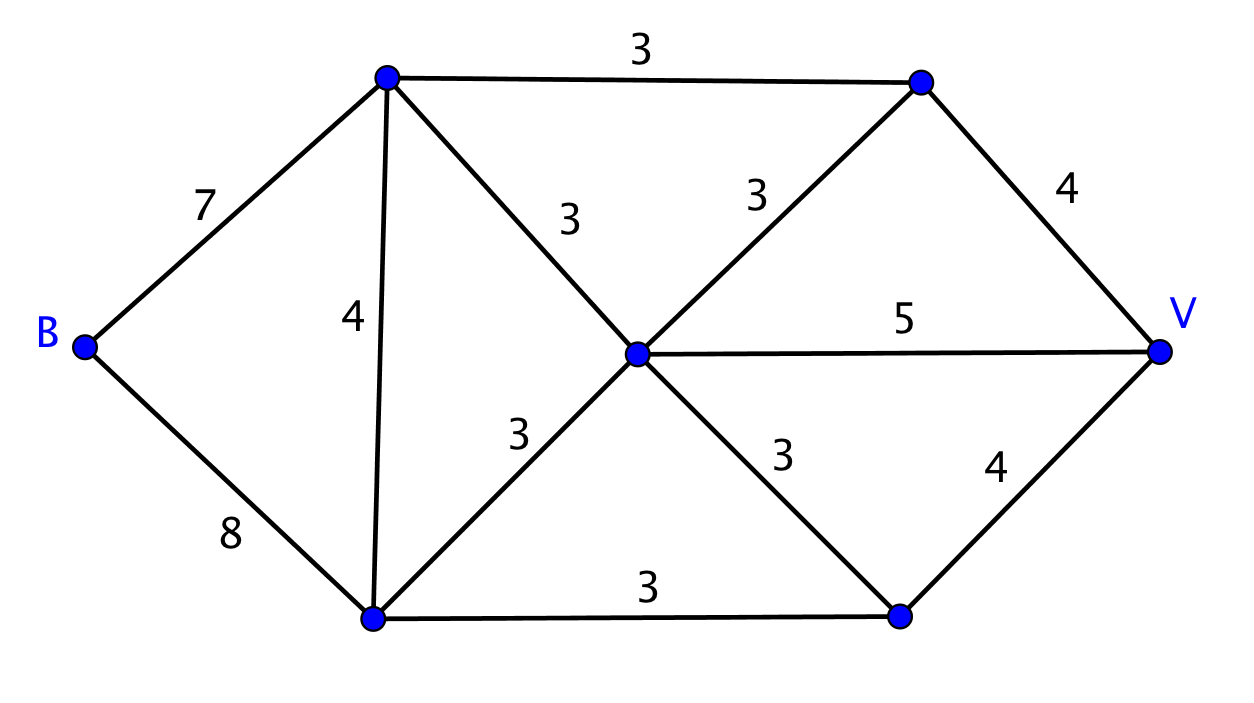
\includegraphics[width=0.6\textwidth, center]{Flaedi3.png}
  \caption*{Netið fyrir verkefni \thesection{}.}
\end{figure}

\section{Tré}
Eitt af eftirfarandi netum (sem eru tré) er hægt að nota sem stærðfræðilíkan af eftirfarandi aðstæðum: þú velur fyrst um tvo forrétti, og síðan um þrjá aðalrétti. Veljið viðeigandi tré og svarið spurningunni: Á hve marga vegu getur samsetta máltíðin verið?

\begin{figure}[h]
\begin{forest}
  for tree={l+=1cm} % increase level distance
  [$\bullet$
    [$\bullet$[$\bullet$][$\bullet$][$\bullet$]]
    [$\bullet$[$\bullet$][$\bullet$][$\bullet$]]
  ]
\end{forest}
\hspace{1cm}
\begin{forest}
  for tree={l+=1cm} % increase level distance
  [$\bullet$
    [$\bullet$[$\bullet$][$\bullet$][$\bullet$][$\bullet$]]
    [$\bullet$[$\bullet$][$\bullet$][$\bullet$][$\bullet$]]
  ]
\end{forest}
\hspace{1cm}
\begin{forest}
  for tree={l+=1cm} % increase level distance
  [$\bullet$
    [$\bullet$[$\bullet$][$\bullet$]]
    [$\bullet$[$\bullet$][$\bullet$]]
  ]
\end{forest}
\caption*{Tré fyrir verkefni \thesection{}.}
\end{figure}

\section{Í skápnum eru herðatré}
Í fataskáp eru skyrtur í 7 litum, 6 mismunandi bindi, jakkar í 3 litum, buxur í 4 litum, sokkar í 5 litum og 2 mismunandi skópör. Á hve marga vegu er hægt að klæða sig, ef maður notar einn hlut af hverju tagi? 

\section{Ósmættanleg tré}
Rifjum upp að net sem hefur enga rás er kallað \textbf{tré}. Teiknið öll \textbf{tré} sem uppfylla samtímis bæði skilyrðin:
\begin{itemize}
    \item það hefur átta hnúta,
    \item en enga hnúta sem hafa gráðuna 2.
\end{itemize}
Alls eru 4 ólík tré -- athugið að tvö net teljast ekki ólík ef það er hægt að „færa“ hnútana í öðru þeirra þannig að það líti eins út og hitt.\\
\textbf{Áskorun}: teiknið líka öll tré sem hafa tíu hnúta en enga hnúta með gráðuna 2. (Svo getið þið skoðað lausnina með því að finna á Youtube viðeigandi atriði út myndinni Good Will Hunting).

\section{Að telja leggi og klíkur}
Rifjum upp að net þar sem allir hnútar tengjast öllum hnútum (það er leggur milli sérhverra tveggja hnúta) nefnist \textbf{fulltengt net}. 
\begin{figure}[h]
    \centering
\begin{tikzpicture}
  %\graph { subgraph K_n [n=8,clockwise,radius=1.5cm] };
  \graph[nodes={draw, circle}, n=5, clockwise, radius=2cm]
  { subgraph K_n [V={A,B,C,D,E}];};
\end{tikzpicture}
\caption*{Netið fyrir verkefni \thesection{}.}
\end{figure}
\begin{enumerate}[(a)]
    \item Hve margir leggir eru í þessu neti? 
    \item Hve margar 3-klíkur í netinu, eða með öðrum orðum, hve margir þríhyrningar þar sem hnútar netsins eru hornpunktarnir (dæmi: ABC)?
    \item Hve margar 4-klíkur (ferhyrningar)?
    \item Hve margar 5-klíkur (fimmhyrningar)?
\end{enumerate}

\section{Fimmur}
\begin{enumerate}[(a)]
\item Ef allir í bekknum gefa öllum hinum fimmu (e. high-five), hve margar fimmur eru gefnar alls? Munið að setja fram almenna reglu og víkka út!
\item Velja á tveggja manna teymi úr hópi 25 nemenda í bekk. Hve mörg slík teymi eru möguleg?
\end{enumerate}

\section{Fjöldi leggja í fulltengdu neti}
Hve margir leggir eru í fulltengdu neti með 10 hnúta? Alhæfið: hve margir leggir eru í fulltengdu neti með $n$ hnúta?

\section{Netafræðingur}
Horfið á viðtal við \href {https://youtu.be/4p2uSjQkW2g} {Mariu Chudnovsky.} Hvaða dæmi tekur hún um hagnýtingu á netafræði? 

\section{Staðalgráða, fjarlægð og þéttni}
Svarið spurningum um netið á eftirfarandi mynd.
\begin{figure}[h!]
\centering
\begin{tikzpicture}
   \node[shape=circle,draw=black] (A) at (0,1.5) {A};
    \node[shape=circle,draw=black] (B) at (2,3) {B};
    \node[shape=circle,draw=black] (C) at (4,3) {C};
    \node[shape=circle,draw=black] (D) at (6,3) {D};
    \node[shape=circle,draw=black] (E) at (6,0) {E};
    \node[shape=circle,draw=black] (F) at (4,0) {F} ;
    \node[shape=circle,draw=black] (G) at (2,0) {G} ;
    \node[shape=circle,draw=black] (H) at (3,1.5) {H} ;
    \node[shape=circle,draw=black] (I) at (5,1.5) {I} ;
    \path [-](A) edge node {} (B);
    \path [-](A) edge node {} (G);
    \path [-](B) edge node {} (G);
    \path [-](B) edge node {} (C);
    \path [-](B) edge node {} (H);
    \path [-](I) edge node {} (E);
    \path [-](H) edge node {} (G);
    \path [-](H) edge node {} (F);
    \path [-](H) edge node {} (C); 
    \path [-](G) edge node {} (F); 
    \path [-](C) edge node {} (D); 
    \path [-](F) edge node {} (F); 
    \path [-](H) edge node {} (C); 
    \path [-](C) edge node {} (F);
    \path [-](I) edge node {} (C);
    \path [-](I) edge node {} (F);
    \path [-](F) edge node {} (E);
    \path [-](I) edge node {} (D);
\end{tikzpicture}
\caption*{Netið fyrir verkefni \thesection{}.}
\end{figure}
\begin{enumerate}[(a)]
    \item \textbf{Staðalgráða hnútar} er skilgreind sem: hve mörg prósent af hinum hnútunum tengjast hnútinum, eða $S(x)=\frac{g(x)}{n-1}$, þar sem $n$ er fjöldi hnúta í netinu og $g(x)$ er gráða hnútarins $x$. Finnið staðalgráðu hnútarins $F$, sem sagt $S(F)$.
    \item \textbf{Fjarlægð milli tveggja hnúta} er skilgreind sem fjöldi leggja í stysta mögulega vegi milli hnútanna. Hver er fjarlægðin milli hnútanna B og E?
    \item \textbf{Þéttni nets} er skilgreint sem hlutfallið milli fjölda leggja og fjölda mögulegra leggja ef allir hnútar tengdust öllum hnútum. Með öðrum orðum er þéttni $\frac{n}{m}$ þar sem $n$ táknar fjölda leggja í netinu, en $m$ táknar fjölda leggja í fulltengdu neti með jafn marga hnúta og netið sem um ræðir. Hver er þéttni netsins sem sýnt er?
    \item Teiknið net sem hefur 5 hnúta og þéttni sem er minni en 40\% og meiri en 10\%.
\end{enumerate}

\section{Vik, þvermál, grenndir}
Hér er ímyndað vinatengslanet á samfélagsmiðli (til dæmis Facebook). Við sleppum því að nota nöfn, notum bara bókstafi. 
\label{sec:streymi}
\begin{figure}[h!]
\centering
\begin{tikzpicture}
   \node[shape=circle,draw=black] (A) at (-6,2) {A};
    \node[shape=circle,draw=black] (B) at (-4.5,0) {B};
    \node[shape=circle,draw=black] (C) at (-5,-2) {C};
    \node[shape=circle,draw=black] (D) at (-3,0) {D};
    \node[shape=circle,draw=black] (E) at (-1,1) {E};
    \node[shape=circle,draw=black] (F) at (0,0) {F} ;
    \node[shape=circle,draw=black] (G) at (1,2) {G} ;
    \node[shape=circle,draw=black] (H) at (2,-1) {H} ;
    \node[shape=circle,draw=black] (I) at (4,-1) {I} ;
    \node[shape=circle,draw=black] (J) at (3,1) {J} ;
    \node[shape=circle,draw=black] (K) at (4,2) {K} ;
    \node[shape=circle,draw=black] (L) at (5,1) {L} ;
    %\path [->](A) (B); 
    \path [-](A) edge node {} (B);
    \path [-](B) edge node {} (C);
    \path [-](A) edge node {} (D);
    \path [-](D) edge node {} (C);
    \path [-](A) edge node {} (E);
    \path [-](D) edge node {} (E);
    \path [-](D) edge node {} (F);
    \path [-](C) edge node {} (F);
    \path [-](E) edge node {} (F);
    \path [-](A) edge node {} (G);
    \path [-](B) edge node {} (D);
    \path [-](C) edge node {} (A);
    \path [-](C) edge node {} (H);
    \path [-](H) edge node {} (F);
    \path [-](H) edge node {} (G);
    \path [-](H) edge node {} (I);
    \path [-](H) edge node {} (J);
    \path [-](J) edge node {} (K);
    \path [-](K) edge node {} (L);
    \path [-](I) edge node {} (J);
    \path [-](J) edge node {} (L);
\end{tikzpicture}
\caption*{Net fyrir verkefni \thesection{}.}
\end{figure}
\begin{enumerate}[(a)]
    \item Ef allar leiðir milli einhverra tveggja hnúta liggja um einhvern tiltekinn hnút $P$, þá kallast $P$ \textbf{hlið}. Hvaða hnútar eru hlið í þessu neti?
    \item \textbf{Hringvik} hnútar táknar mestu fjarlægð frá einhverjum öðrum hnúti (talið í fjölda leggja). Hvaða hnútar hafa mesta hringvikið og hvaða hnútar hafa minnsta hringvikið?
    \item \textbf{Þvermál} nets er stærsta hringvikið í netinu og \textbf{radíus} nets er minnsta hringvikið í því. Hvert er þvermál netsins og hver er radíusinn?
    \item Hver er minnsti mögulegi hópur af vinum sem gæti póstað einhverju þannig að allir gætu séð það?
    \item \textbf{Grennd} hnútar eru allir hnútar sem tengjast þeim hnúti. Hver er grennd hnútarins $H$?
    \item Hver er minnsti mögulegi hópur vina sem gæti póstað einhverju þannig að allir hafa annaðhvort póstað því sjálfir eða meirihluti vina þeirra póstaði því?
    \item \textbf{Þéttleikastuðull} einstaklings (hnútar) $X$ eru líkindin á því að tveir einstaklingar valdir af handahófi úr grennd $X$ séu vinir. Hver er þéttleikastuðull $D$?
    \item Hugsum okkur nú að netið tákni vini sem umgangast mikið. Segjum að upp komi smitandi sjúkdómur. Ef þú ættir að bólusetja einhverja þrjá til að takmarka útbreiðsluna sem mest, hverja myndirðu bólusetja?
\end{enumerate}

\section{Hve mörg einföld net?}
\textbf{Einfalt net} er net þar sem engar lykkjur eru, og aldrei meira en einn leggur milli tveggja hnúta.
Hve mörg mismunandi einföld net með þremur hnútum eru til? En með fjórum hnútum? Og svo framvegis. 

\section{Einn--margir}
Hér eru þrjú dæmi um einföld net þar sem einn hnútur (A) getur tengst hinum hnútunum eða ekki. Hnútar í efri röðinni tengjast ekki innbyrðis.

\begin{figure}[h]
  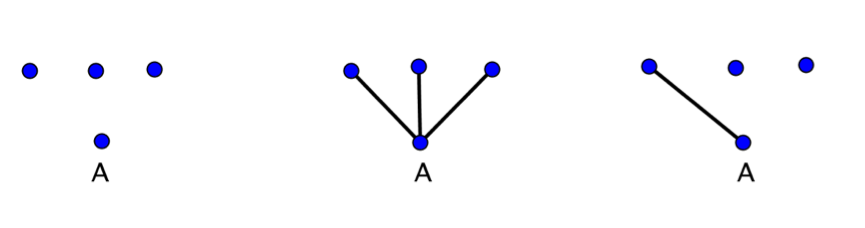
\includegraphics[width=0.5\textwidth, center]{1-3net.png}
  \caption*{Net fyrir verkefni \thesection{}.}
\end{figure}
\begin{enumerate}[(a)]
    \item Hve mörg net eins og þessi eru möguleg?
    \item Hve mörg net væru möguleg ef það væru 1, 2, eða 4 hnútar í efri röðinni?
    \item Alhæfið: hve mörg net væru möguleg ef það væru $n$ hnútar í efri röðinni?
\end{enumerate}

\section{Pítsudæmið}
\begin{enumerate}[(a)]
\item Hve margar mismunandi pítsur er hægt að panta ef það eru 4 áleggstegundir í boði (og ekki má velja sama álegg tvisvar)?
\item Hvað ef það eru 5 áleggstegundir? En fleiri?
\end{enumerate}

\section{Vinir og ókunnugir} 
Látið reyna á eftirfarandi tilgátu með því að teikna tengslanet:
\begin{quote}
Ef sex manneskjur eru í veislu þá er öruggt að einhverjir þrír þekkjast allir innbyrðis eða einhverjir þrír þekkjast ekki innbyrðis (engin þeirra þekkir neina af hinum tveimur).
\end{quote}
Hér er önnur leið til að setja fram sömu tilgátu:
\begin{quote}
Segjum að við höfum fulltengt net með sex hnútum. Ef við litum sérhvern hnút rauðan eða bláan, þá verður einhver þríhyrningur með bláum hnútum eða einhver þríhyrningur með rauðum hnútum.
\end{quote}
Haldið þið að þetta sé rétt? Hvernig eru þetta sömu tilgáturnar?\\
\textbf{Áskorun:} Svarið spurningunni og sýnið fram á svarið.\\
Athugasemd: Svarið við þessari spurningu er svo fræg að hún á sér sérstakt nafn og Wikipediu-síðu, \href {https://en.wikipedia.org/wiki/Theorem_on_friends_and_strangers} {Theorem on friends and strangers.} 

\section{Partí}
\label{sec:skuffureglan}
Hugsið ykkur að þið séuð í partíi með hundrað manns. Einhver fær þá hugmynd að komast að því hver er vinur hvers í partíinu. Viðkomandi sýnir þér listann og þú tekur eftir því að tvær manneskjur eiga nákvæmlega jafn marga vini. Þér dettur í hug tilgáta: í öllum partíum eru alltaf að minnsta kosti tvær manneskjur sem eiga nákvæmlega jafn marga vini í partíinu. Er þessi tilgáta rétt?
Athugasemd: Hér má reyna að byrja á því að skoða partí með 3, 4, og 5 manns. Jafnvel tveimur, eða einum! Það gæti gefið hugmyndir.

\section{Einn sem þekkir alla}
Kannið tilgátuna: 
\begin{quote}
Ef hópur fólks er þannig að sérhver tvö í hópnum eiga nákvæmlega einn sameiginlegan vin í hópnum, þá er einhver einn í hópnum sem er vinur allra hinna.
\end{quote}
Teiknið einhver net til að rannsaka þetta.

\section{Ferðalög í neti}
\begin{figure}[h]
    \centering
\begin{tikzpicture}
  %\graph { subgraph K_n [n=8,clockwise,radius=1.5cm] };
  \graph[nodes={draw, circle}, n=5, clockwise, radius=1.7cm]
  { subgraph K_n [V={A,B,C,D,E}];};
\end{tikzpicture}
\caption*{Net fyrir verkefni \thesection{}.}
\end{figure}
\begin{enumerate}[(a)]
    \item Hve margar ólíkar ferðir með einum legg eru í netinu? (Tvö dæmi: A-E og E-A).
    \item Hve margar ólíkar ferðir með tveimur ólíkum leggjum?
    \item Hve margar ólíkar ferðir með þremur ólíkum leggjum?
    \item Hve margar ólíkar ferðir með fjórum ólíkum leggjum?
    \item Hve margar ólíkar ferðir með tveimur leggjum ef það má endurtaka leggi?
    \item Hve margar ólíkar ferðir með þremur leggjum ef það má endurtaka leggi?
    \item Hve margar ólíkar ferðir með fjórum leggjum ef það má endurtaka leggi?
\end{enumerate}

\section{Farandsölumaðurinn}
\label{sec:travelling}
Mjög frægt verkefni úr netafræði heitir \textit{The travelling salesman problem} á ensku, við gætum kallað það „höfuðverk farandsölumannsins“. Það snýst um að finna hagkvæmustu (eða stystu) leiðina til að koma við á mörgum áfangastöðum og snúa aftur heim. \\
Á myndinni táknar hver hnútur borg og leggirnir tákna leiðina á milli þeirra og tölurnar tákna kostnað (þúsundir króna) við að fara þann legg. Hugsaðu þér að þú þurfir að koma við í öllum borgunum og enda á sama stað og þú byrjar. Net þar sem hverjum legg er úthlutuð tala (sem getur táknað vegalengd, kostnað, eða eitthvað annað) er nefnt \textbf{vegið net}.

\begin{figure}[h]
  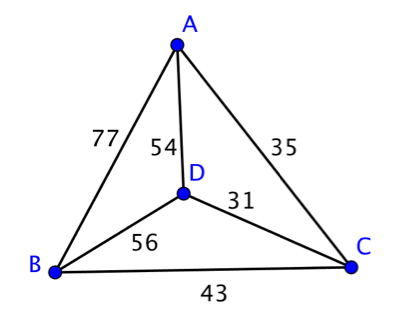
\includegraphics[width=0.4\textwidth, center]{tsp1.png}
  \caption*{Net fyrir verkefni \thesection{}.}
\end{figure}

\begin{enumerate}[(a)]
    \item Hve margar mögulegar leiðir eru til að ferðast til allra borganna einu sinni? Skráðu þær allar og kostnaðinn við þær. 
    \item Hvernig er ódýrast að fara í ferðalag og koma við í hverri borg einu sinni? 
\end{enumerate}

\section{Sex skrefa aðskilnaður (six degrees of separation)}
\label{sec:sixdegrees}
\begin{enumerate}[(a)]
\item Hvað þekkir þú margar manneskjur? Til dæmis á Facebook.
\item Leggðu mat á það hvað þeir sem þú þekkir þekkja marga sem þú þekkir ekki. (Þetta er auðvitað bara einhvers konar skynsamleg ágiskun um meðalfjölda.)
\item Segjum að þeir sem þú þekkir séu í fjarlægðinni 1, (einn „hlekkur”), en þeir sem þeir þekkja, og þú ekki, séu í fjarlægðinni 2 (tveir hlekkir) frá þér. Notaðu tölurnar sem þú fékkst að ofan til að meta hvað margir eru einum, tveimur, 3, 4, 5 og 6 hlekkjum frá þér.
\item Ein kenning segir að hægt sé að tengja sérhverjar tvær manneskjur á jörðinni hvor við aðra í sex eða færri hlekkjum. Hvað heldur þú um það? (Gefið rökstutt svar.) Þessi kenning gengur undir heitinu „Six degrees of separation“ og er hægt að gúgla.
\end{enumerate}

\section{Vatn, hiti og rafmagn}
\label{sec:vatnhiti}
Leggja þarf lagnir fyrir kalt vatn, vatnsveitu og rafmagnsveitu í þrjú hús.

\begin{figure}[h]
  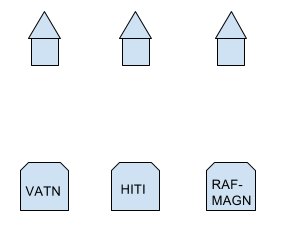
\includegraphics[width=0.4\textwidth, center]{Vatnhiti.png}
  \caption*{Verkefni \thesection{}.}
\end{figure}

\noindent 
Er hægt að gera það án þess að nokkurs staðar þurfi ein lögn að liggja yfir aðra?

\section{Lagnet}
Í netafræði skiptir engu máli hvar hnútarnir eru teiknaðir, það eina sem skiptir máli er hvaða hnútar tengjast með leggjum. Net nefnist \textbf{lagnet} ef hægt er að teikna það án þess að leggir skarist (fari ofan í hvorn annan). Síðasta verkefni var semsagt um það hvort net væri lagnet.

Hvernig er hægt að teikna eftirfarandi þrjú net þannig að engir leggir skarist? Það má einfaldlega hugsa sér að maður færi hnútana (en passi að leggirnir slitni ekki).
\begin{figure}[h]
  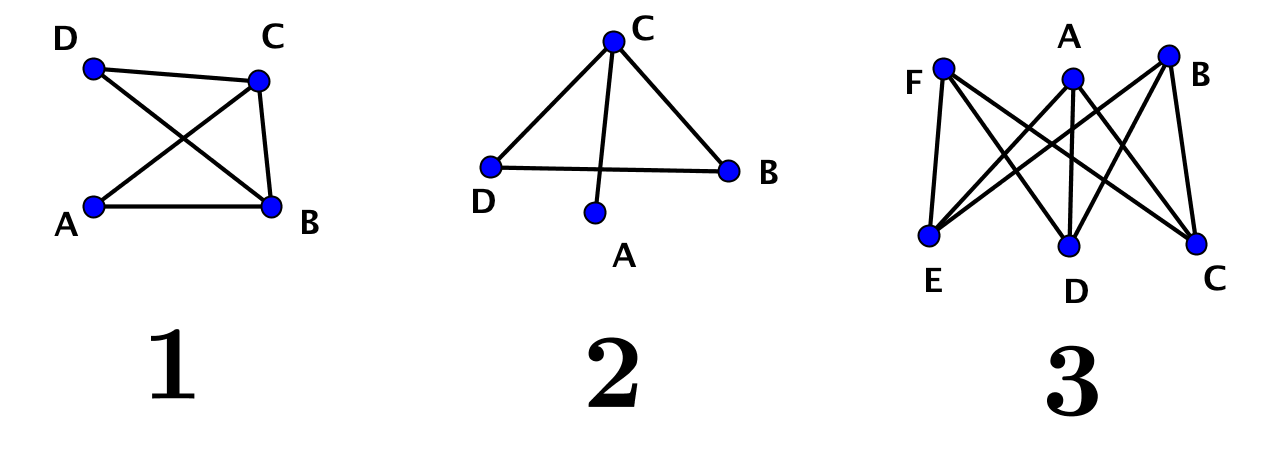
\includegraphics[width=0.7\textwidth, center]{3Lagnet.png}
  \caption*{Net fyrir verkefni \thesection{}.}
\end{figure}

(Það er hægt að teikna net 1 og 2 án þess að leggir skarist, þau eru lagnet, en ekki net 3, sem er þá ekki lagnet.)

\section{Svæðaskipting}
Ef við teiknum lagnet þá skiptir það fletinum (pappírnum, skjánum) í svæði (eins og leggirnir væru girðingar eða landamæri). Hefð er fyrir því að telja svæðið „fyrir utan“ með. Net 1 hér að neðan skiptir fletinum í 4 svæði, en í hve mörg svæði skipta net 2 og 3 fletinum?

\begin{figure}[h]
  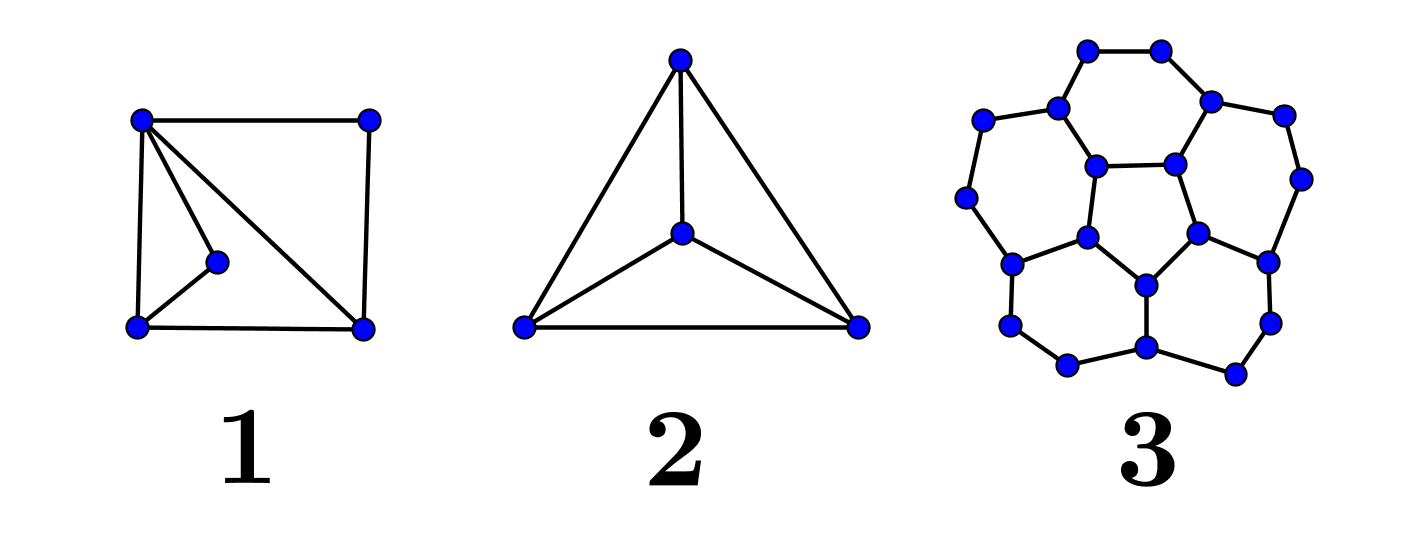
\includegraphics[width=0.6\textwidth, center]{3Svaedi_lagnet.png}
  \caption*{Lagnet fyrir verkefni \thesection{}.}
\end{figure}

\section{Leggir, hnútar og svæði}
\label{sec:eulerchar}
Til er regla sem tengir saman fjölda hnúta, leggja og svæða. Verkefnið er að finna út hvernig fjöldi leggja, hnúta og svæða tengjast. Til að aðstoða er ykkur bent á að gera töflu yfir nokkur net, þar sem fram koma: fjöldi leggja, fjöldi hnúta og fjöldi svæða sem netið skiptir fletinum í. Þið getið teiknað ykkar eigin lagnet, og/eða notað þessi (og netin í verkefninu á undan).
\noindent
\textbf{Áskorun}: rökstyðjið eða sannið regluna.

\begin{figure}[h]
  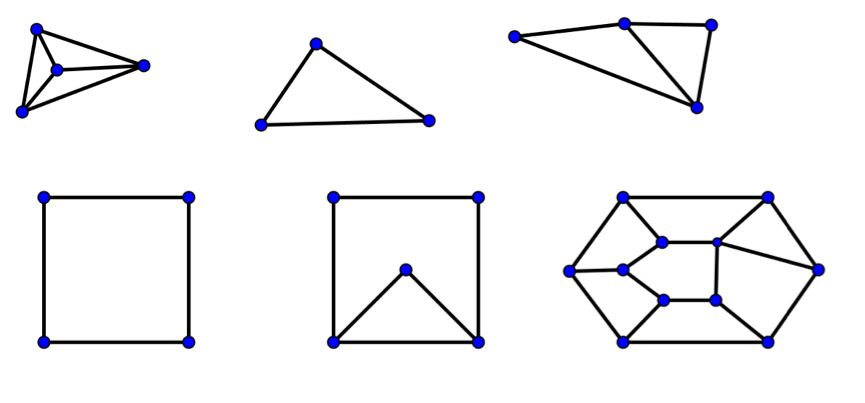
\includegraphics[width=0.6\textwidth, center]{Nokkur_lagnet.png}
  \caption*{Lagnet fyrir verkefni \thesection{}.}
\end{figure}

\section{Áskorun: um yfirborð fótbolta}
\label{sec:fotbolti}
Reglan um fjölda hnúta, leggja og svæða gildir ekki bara á flötum pappír, heldur líka á kúluyfirborði. Að því gefnu að yfirborð gamaldags fótbolta sé gert úr fimm- og sexhyrningum, sýnið fram á að fjöldi fimmhyrninga er 12 og fjöldi sexhyrninga er 20. Stærð boltans skiptir ekki máli! [Þetta er mjög krefjandi verkefni.]

\begin{figure}[h]
  
\includegraphics[width=0.2\textwidth, center]{bolti.jpg}
  \caption*{Fótbolti fyrir verkefni \thesection{}.}
\end{figure}

\section{Hamilton--net}
Net er sagt vera Hamilton-net ef hægt er að fara gegnum það þannig að maður komi við í hverjum einasta hnúti nákvæmlega einu sinni og endi á sama stað og maður byrjaði. Eru eftirfarandi net Hamilton-net, annað eða bæði?

\begin{figure}[h]
  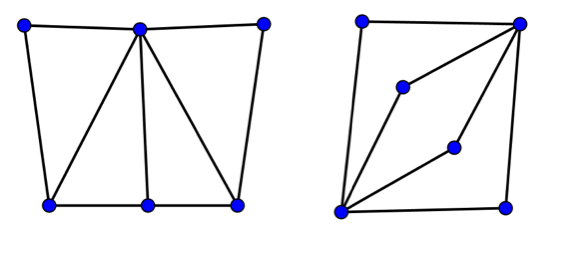
\includegraphics[width=0.5\textwidth, center]{Hamiltonnet1.png}
  \caption*{Hamilton-net? (Sjá verkefni \thesection{}).}
  
\end{figure}

\section{Litun landakorts}
\label{sec:landakort}
Hve marga liti þarf (í minnsta lagi) til að lita þetta landakort þannig að engin lönd með sameiginleg landamæri séu í sama lit?

\begin{figure}[h]
  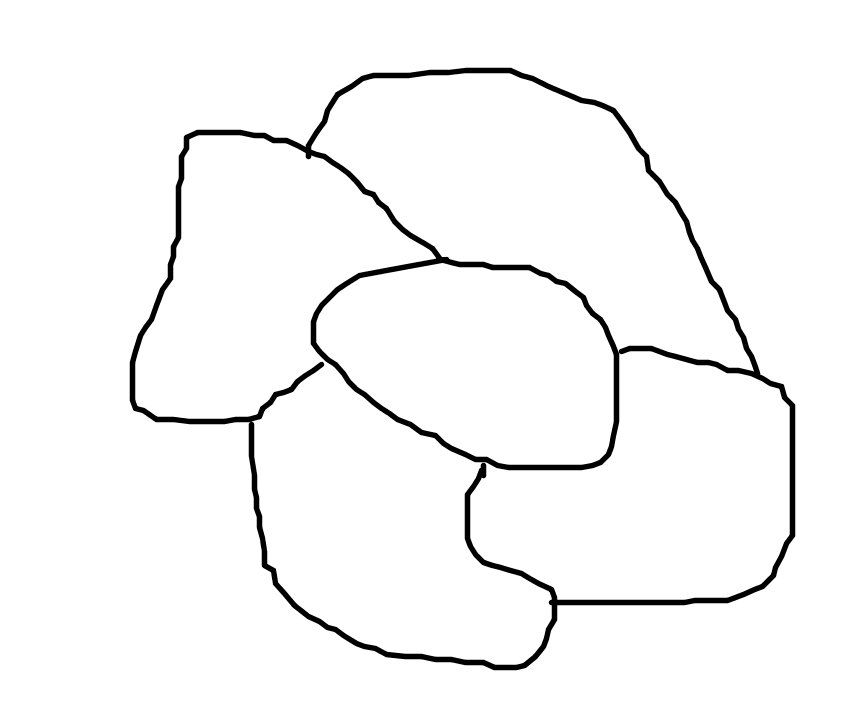
\includegraphics[width=0.3\textwidth, center]{litakort.png}
  \caption*{Landakort fyrir verkefni \thesection{}.}
\end{figure}

\section{Litun næstum Evrópu}
Hve marga liti þarf til að lita þetta landakort þannig að engin lönd með sameiginleg landamæri séu í sama lit? (Það er í lagi að tvö lönd hafi sama lit ef „landamærin“ eru bara einn punktur.)

\begin{figure}[h]
  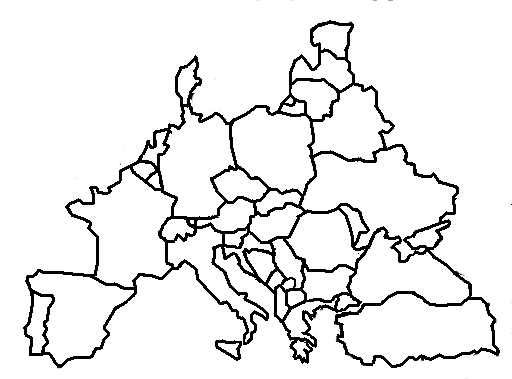
\includegraphics[width=0.5\textwidth, center]{Evropa.png}
  \caption*{Kort af (hluta) af Evrópu, sjá verkefni \thesection{}.}
\end{figure}

\section{Litun neta}
Hve marga liti þarf til að lita hnútana í eftirfarandi netum, þannig að engir tveir hnútar í sama lit tengist? (Athugið, hér er spurt um litun hnúta, ekki svæða.)
\begin{figure}[h]
\centering
\begin{tikzpicture}
\graph[nodes={draw, circle}, cycle, n=3, clockwise, radius=2cm]
    {
    1/, 2/, 3/
    };
  \node[shape=circle,draw=black] (D) at (0,0) {};
  \path [-](D) edge node {} (1);
  \path [-](D) edge node {} (2);
  \path [-](D) edge node {} (3);
  
\begin{scope}[shift={(5,0)}]
\graph[nodes={draw, circle}, cycle, n=4, clockwise, radius=2cm]
    {
    1/, 2/, 3/, 4/
    };
  \node[shape=circle,draw=black] (D) at (0,0) {};
  \path [-](D) edge node {} (1);
  \path [-](D) edge node {} (2);
  \path [-](D) edge node {} (3);
  \path [-](D) edge node {} (4);
 \end{scope}
 
\begin{scope}[shift={(10,0)}]
\graph[nodes={draw, circle}, cycle, n=10, clockwise, radius=2cm]
    {
    1/, 2/, 3/, 4/, 5/, 6/, 7/, 8/, 9/, 10/
    };
  \node[shape=circle,draw=black] (D) at (0,0) {};
  \path [-](D) edge node {} (1);
  \path [-](D) edge node {} (2);
  \path [-](D) edge node {} (3);
  \path [-](D) edge node {} (4);
  \path [-](D) edge node {} (5);    
  \path [-](D) edge node {} (6);
  \path [-](D) edge node {} (7);
  \path [-](D) edge node {} (8);
  \path [-](D) edge node {} (9);
  \path [-](D) edge node {} (10); 
  \end{scope}
\end{tikzpicture}
\caption*{Netin fyrir verkefni \thesection{}.}
\end{figure}

\section{Kóðar}
Öll stafræn samskipti með tölvum, símum eða öðrum tækjum fara þannig fram að fyrst er skilaboðunum (hvort sem það er hljóð, texti eða myndir) breytt í runu af táknunum 0 og 1. Margskonar tækni er á bakvið það hvernig svona runur eru sendar þannig að þær brenglist ekki á leiðinni. Til þess að rannsaka svona merkjasendingar þurfti að búa til hugtak sem „mælir“ hve langt er á milli tveggja runa af táknum. Til dæmis hlýtur að vera lengra á milli 0000 og 1111 heldur en á milli 1100 og 1101. Netafræði nýtist í þessum fræðum ef við hugsum okkur að tvær táknarunur tengist ef þær eru eins fyrir utan eitt tákn (eins og 1100 og 1101). Verkefnið er að teikna netið sem sýnir allar táknarunur með þremur táknum (sem eru 0 eða 1).

\section{Spírur (leikur fyrir tvo)}
Þennan leik má leika með hvaða fjölda af hnútum sem er, en við byrjum á að nota þrjá hnúta. Tveir leikmenn skiptast á að leika. Hægt er að leika tvenns konar leiki:
\begin{enumerate}[(a)]
\item tengja saman tvo hnúta og búa til nýjan hnút á leiðinni, eða
\item búa til nýjan hnút sem tengist gömlum hnúti með tveimur leggjum.
Svo upphafsstaðan eru þrír ótengdir hnútar, og næsta staða gæti verið til dæmis A eða B.
\end{enumerate}

\begin{figure}[h]
  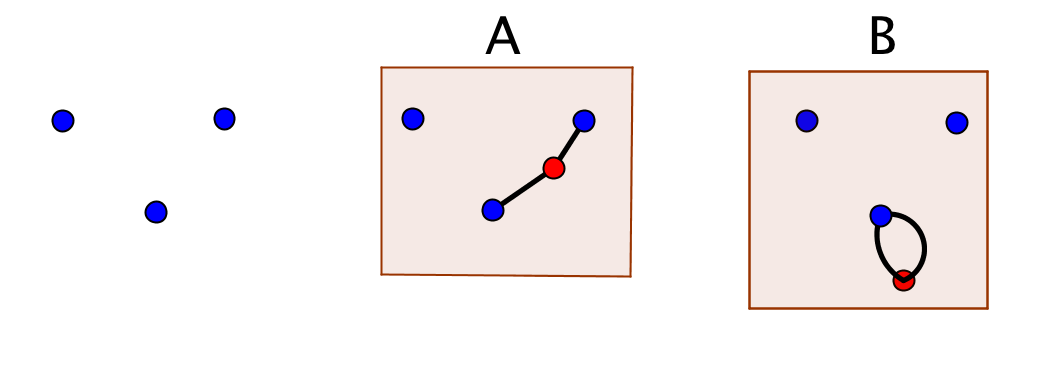
\includegraphics[width=0.7\textwidth, center]{Sprouts1.png}
  \caption*{Frá upphafsstöðu er hægt að komast í stöðu A eða B (eða aðrar eins), sjá verkefni \thesection{}.}
\end{figure}

Auk þess eru eftirfarandi reglur: 
\begin{enumerate}
\item Það má ekki teikna legg sem sker annan legg (fer „yfir“ eða „ofan í“ annað strik). 
\item Hnútur má ekki hafa fleiri en þrjá leggi (hæsta leyfilega gráða hnútar er 3). Þannig að til dæmis er ekki hægt að gera neitt við hnúta A og B í þessari stöðu hér fyrir neðan.
\item Sá vinnur sem teiknar síðasta legginn!
\end{enumerate}

\begin{figure}[h]
  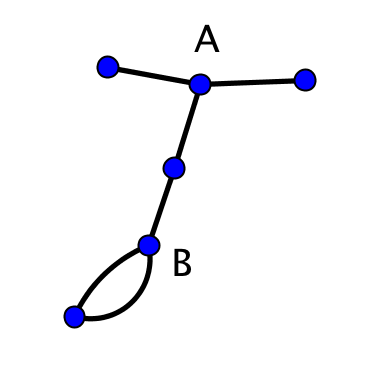
\includegraphics[width=0.3\textwidth, center]{Sprouts2.png}
  \caption*{A og B eru „úr leik“}
\end{figure}

Verkefnið er að 
\begin{enumerate}
\item leika þennan leik við einhvern til að fá tilfinningu fyrir honum.
\item Finna út hver hefur tilhneigingu til að vinna: sá sem byrjar eða hinn?
\item  Eru einhverjar sigurleiðir (taktík, strategía)?
\item Hve langur getur leikurinn orðið (talið í fjölda skipta sem hver gerir)?
\end{enumerate}

Athugasemd:
Leikur með þremur hnútum getur mest orðið 8 leikir. (Í hverju skrefi fækkar mögulegum leggjum sem hægt væri að bæta við um (amk) 1.) Sá sem hefur leikinn getur unnið ef upphafsfjöldi hnúta er 3, 4, eða 5, en hann tapar ef fjöldinn í upphafi er 1 eða 2, eða 6, 7, 8. Engin auðveld leið er til að sýna fram á þetta, og almennt er ekki þekkt hver getur tryggt sér sigur, en tilgátan sem stendur er: sá sem byrjar getur unnið ef fjöldi hnúta í upphafi gefur afganginn 3, 4, eða 5 þegar deilt er með 6. 




%%%%%%%%%%%%%%%%%%%%%%%%%%%%%%%%%%%%%%%%%%%%%%%%%%
%%%%%%%%%%%%%%%%%%%%%%%%%%%%%%%%%%%%%%%%%%%%%%%%%%
%%%%%%%%%%%%%%%%%%%%%%%%%%%%%%%%%%%%%%%%%%%%%%%%%%
%%%%%%%%%%%%%%%%%%%%%%%%%%%%%%%%%%%%%%%%%%%%%%%%%%

\chapter*{Fróðleikur og vísbendingar}
\label{chap:frodleikur}
\section*{\ref{sec:fyrstanet}}
Hægt er að \textbf{setja fram} sömu upplýsingar og sömu stærðfræði á marga mismunandi vegu. Hér eru nokkrar \textbf{framsetningar} á þeim aðstæðum sem dæmið fjallar um:
    \begin{figure}[h]
  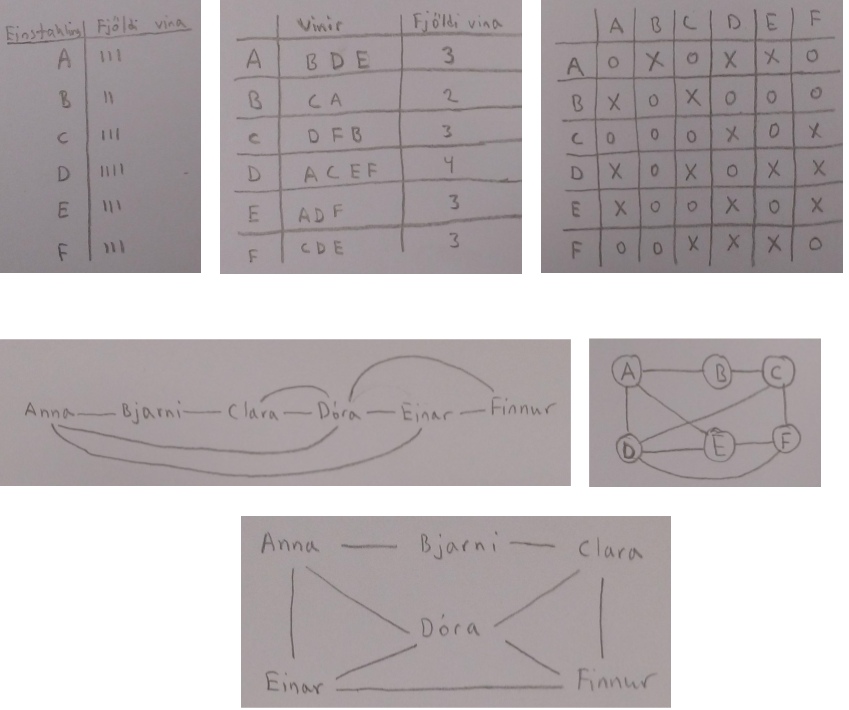
\includegraphics[scale=0.5, center]{Fyrstunet.png}
  \caption*{Ólíkar framsetningar í verkefni \ref{sec:fyrstanet}}
\end{figure}
Skoðið þessar ólíku framsetningar. Hverjar þeirra innihalda allar upplýsingar um aðstæðurnar og hverjar ekki? Hverjar eru gagnlegastar að ykkar mati? Takið eftir að alls staðar er gert ráð fyrir því að það séu engin vinatengsl sem ekki voru talin upp í dæmatextanum (þótt það standi ekki að það geti ekki verið önnur).

\section*{\ref{sec:vina}}
Vinaþversögnin á uppruna sinn í grein frá 1991, \href{https://dx.doi.org/10.1086\%2F229693}{Why your friends have more friends than you do} eftir bandaríska félagsfræðinginn Scott L. Feld. Sú regla að meðalfjöldi vina er minni en eða jafn meðalfjölda vina vina er stærðfræðiregla og gildir um öll tengslanet og það er hægt að sanna regluna.

\section*{\ref{sec:skuffureglan}}
Vísbending: Þetta verkefni er hægt að leysa með „skúffureglunni“ og með því að athuga að ef það eru $n$ gestir í partíinu þá gildir: 
\begin{enumerate}
\item maður getur þekkt allt frá $0$ og upp í $n-1$ gesti (maður telur sjálfan sig ekki með til vina sinna);
\item ef einhver þekkir engan er enginn sem þekkir alla, og ef einhver þekkir alla, þá er engin sem þekkir engan.
\end{enumerate}
Þetta þýðir að mögulegar tölur yfir fjölda vina eru einum færri en fjöldi gesta (ef einhver þekkir alla, þá eru möguleikarnir frá $1$ upp í $n-1$ en ef enginn þekkir alla, þá eru möguleikarnir frá $0$ upp í $n-2$).

\section*{\ref{sec:travelling}}
Til eru heilu bækurnar helgaðar þessu verkefni enda skiptir lausn þess gríðarlegu máli. Verkefnið kemur við sögu í skipulagi strætisvagnaleiða, skipaferða, flugleiða, vörudreifingu, framleiðslu á tölvuörflögum, og kemur við sögu í rannsóknum á DNA erfðaefni. Engin aðferð er til sem leysir slík verkefni bæði fljótt og fullkomlega jafnvel þótt tölvur séu notaðar, en margar aðferðir eru til sem finna nokkuð góða lausn á stuttum tíma. Mikið efni er til um þetta verkefni á netinu. Ef þér tekst að búa til almenna aðferð til að leysa það hratt (það þarf dálitla stærðfræðiþekkingu til að skilja hvað „hratt“ þýðir í þessu samhengi) þá geturðu innheimt eina milljón dollara í verðlaun frá Clay-stofnuninni (sjá \href{https://plus.maths.org/content/travelling-salesman}{vefsíðu Clay-stofnunarinnar}).

\section*{\ref{sec:sixdegrees}}
Um sex gráðu aðskilnað: Tveir einstaklingar á Facebook tengjast að meðaltali með 3.5 milliliðum (2016). Sjá \href{https://research.fb.com/three-and-a-half-degrees-of-separation/}{Three and a half degrees of separation.} Til er vefsíða sem finnur út hve margir „hlekkir“ eru á milli kvikmyndaleikara, hún heitir \href{https://oracleofbacon.org/}{The oracle of Bacon}, til heiðurs leikaranum Kevin Bacon. (Svo ef leikari hefur Bacon-töluna 1, þá hefur hann leikið í mynd með Kevin Bacon. Ef hann hefur Bacon-töluna 2, þá hefur hann leikið í mynd með einhverjum sem hefur leikið í mynd með Kevin Bacon, og svo framvegis.)

\section*{\ref{sec:vatnhiti}}
Þetta verkefni er óleysanlegt, eins og lesa má um á svari vísindavefsins \href{http://visindavefur.is/svar.php?id=53461}{„Gefnir eru þrír hringir og þrír kassar. Er hægt að tengja hvern hring við hvern kassa með strikum án þess að strikin skerist?“} Þar má fræðast meira almennt um það hverskonar net eru lagnet og hver ekki.

\section*{\ref{sec:eulerchar}}
Jafnan sem lýsir samhenginu milli fjölda hnúta, leggja og svæða í lagneti heitir jafna Eulers, og má lesa um 

\section*{\ref{sec:fotbolti}}
Vísbending: Notum $l$ fyrir fjölda leggja, $h$ fyrir fjölda hnúta, og $s$ fyrir fjölda svæða. Setning Eulers segir að $h-l+s=2$. Segjum nú að fjöldi fimmhyrninga sé $a$ og fjöldi sexhyrninga sé $b$. Við vitum þá að $s=a+b$. Nú þarf að finna samband milli fjölda svæða og fjölda leggja og hnúta. Það er hægt að gera á ýmsa vegu. Til dæmis: hvernig tengist fjöldi hnúta og fjöldi fimm- og sexhyrninga? Jú, sérhver hnútur er hornpunktur eins fimmhyrnings, og sérhver fimmhyrningur hefur fimm hornpunkta, svo $5a=h$. Einnig er hver hnútur hornpunktur tveggja sexhyrninga, og hver sexhyrningur hefur sex hornpunkta svo $h= \frac{6b}{2}=3b$. Ef þessi leið er farin þarf núna að finna samband milli fjölda leggja og fjölda hnúta, og eftir það er hægt að reikna dæmið með jöfnu Eulers. 

\section*{\ref{sec:landakort}}
Um litun landakorta: Sú tilgáta var sett fram á 19. öld að aldrei þyrfti fleiri en fjóra liti til að lita landakort. (Þessi regla heitir fjögurra lita setningin í stærðfræði eða \textit{the four color theorem} á ensku.) Það var hins vegar ekki fyrr en árið 1976 að tókst að sanna tilgátuna, og það þurfti tölvu til þess að aðstoða við sönnunina með því að fara gegnum þúsundir möguleika sem sýnt var fram á að þyrfti að skoða. Í þessu myndbandi er skemmtilega sagt frá fjögurra lita setningunni: \href{https://youtu.be/NgbK43jB4rQ}{The Four Color Map Theorem - Numberphile}.


\chapter*{Um stærðfræðilegt inntak þessa rits}
Sjálft stærðfræðilega inntakið í þessu riti er einkum um eftirfarandi atriði:
\begin{enumerate}
\item Tengsl heildargráðu nets við fjölda leggja og hvað þá er hægt að segja um heildargráðu nets.
\item Regla um mögulegan fjölda oddahnúta.
\item Einkenni neta sem hafa Euler-rásir og Euler-vegi.
\item Talningar á leggjum, hnútum og klíkum í ýmsum netum.
\item Að nota net sem stærðfræðileg líkön af ýmsum aðstæðum.
\item Að leysa ýmsar þrautir með því að nýta sér netaframsetningu.
\end{enumerate} 

\end{document}


% you can color the countries of a map with alternating colors if and only if you can draw the whole map with a single curve (the ocean must count as a country). Can you see the curve in my drawing?!
% sjá https://twitter.com/yougetaquote/status/1240065705757642752

